\documentclass{standalone}
\usepackage{pgfplots}
\usepackage{tikz}
\usepackage{siunitx}
\begin{document}
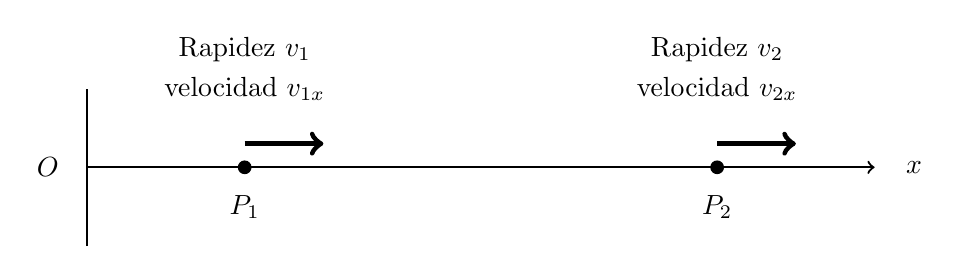
\begin{tikzpicture}[font=\normalsize]
    \draw [thick, ->] (0,0) -- (10, 0) node [at end, pos=1.05pt] {$x$};
    \draw [thick] (0, -1) -- (0, 1);
    \node at (-0.5, 0) {$O$};
    \draw [fill] (2, 0) circle (0.08);
    \node at (2, -0.5) {$P_{1}$};
    \draw [line width=0.7mm, ->] (2, 0.3) -- (3, 0.3);
    \node at (2, 1) {velocidad $v_{1x}$};
    \node at (2, 1.5) {Rapidez $v_{1}$};
    
    \draw [fill] (8, 0) circle (0.08);
    \node at (8, -0.5) {$P_{2}$};
    \draw [line width=0.7mm, ->] (8, 0.3) -- (9, 0.3);
    \node at (8, 1) {velocidad $v_{2x}$};
    \node at (8, 1.5) {Rapidez $v_{2}$};
\end{tikzpicture}
\end{document}